\documentclass[11pt, a4paper, twoside]{article}   	% use "amsart" instead of "article" for AMSLaTeX format

\usepackage{geometry}                		% See geometry.pdf to learn the layout options. There are lots.
\usepackage{pdfpages}
\usepackage{caption}
\usepackage{minted}
\usepackage[german]{babel}			% this end the next are needed for german umlaute
\usepackage[utf8]{inputenc}
\usepackage{color}
\usepackage{graphicx}
\usepackage{titlesec}
\usepackage{fancyhdr}
\usepackage{lastpage}
\usepackage{hyperref}
% http://www.artofproblemsolving.com/wiki/index.php/LaTeX:Symbols#Operators
% =============================================
% Layout & Colors
% =============================================
\geometry{
   a4paper,
   total={210mm,297mm},
   left=20mm,
   right=20mm,
   top=20mm,
   bottom=30mm
 }	

\definecolor{myred}{rgb}{0.7,0.3,0.4}
\definecolor{mygreen}{rgb}{0,0.6,0}
\definecolor{mygray}{rgb}{0.5,0.5,0.5}
\definecolor{mymauve}{rgb}{0.58,0,0.82}

\setcounter{secnumdepth}{4}

% the default java directory structure and the main packages
\newcommand{\appRoot}{../source/AmazingRace/app}
\newcommand{\javaRoot}{\appRoot/src/main/java/at/fh/ooe/moc5/amazingrace}
\newcommand{\resRoot}{\appRoot/src/main/res}
\newcommand{\activityRoot}{\javaRoot/activity}
\newcommand{\adapterRoot}{\javaRoot/adapter}
\newcommand{\jsonModelRoot}{\javaRoot/model/json}
\newcommand{\taskModelRoot}{\javaRoot/model/task}
\newcommand{\viewModelRoot}{\javaRoot/model/view}
\newcommand{\serviceRoot}{\javaRoot/service}
\newcommand{\utilRoot}{\javaRoot/util}
\newcommand{\watcherRoot}{\javaRoot/watcher}
\newcommand{\layoutRoot}{\resRoot/layout}
\newcommand{\valuesRoot}{\resRoot/values}
\newcommand{\manifestsRoot}{\appRoot/src/main}
\newcommand{\imagesRoot}{images}

% =============================================
% Code Settings
% =============================================
\newenvironment{code}{\captionsetup{type=listing}}{}
\newmintedfile[javaSourceFile]{java}{
	linenos=true, 
	frame=single, 
	breaklines=true, 
	tabsize=2,
	numbersep=5pt,
	xleftmargin=10pt,
	baselinestretch=1,
	fontsize=\footnotesize
}
\newmintinline[inlineJava]{java}{}
\newminted[javaSource]{java}{
	breaklines=true, 
	tabsize=2,
	autogobble=true,
	breakautoindent=false
}
\newmintedfile[xmlSourceFile]{xml}{
	linenos=true, 
	frame=single, 
	breaklines=true, 
	tabsize=2,
	numbersep=5pt,
	xleftmargin=10pt,
	baselinestretch=1,
	fontsize=\footnotesize
}
\newmintedfile[propertiesFile]{properties}{
	linenos=true, 
	frame=single, 
	breaklines=true, 
	tabsize=2,
	numbersep=5pt,
	xleftmargin=10pt,
	baselinestretch=1,
	fontsize=\footnotesize
}
% =============================================
% Page Style, Footers & Headers, Title
% =============================================
\title{Übung 3}
\author{Thomas Herzog}

\lhead{Übung 3}
\chead{}
\rhead{
\includegraphics[scale=0.10]{FHO_Logo_Students.jpg}}

\lfoot{S1310307011}
\cfoot{}
\rfoot{ \thepage / \pageref{LastPage} }
\renewcommand{\footrulewidth}{0.4pt}
% =============================================
% D O C U M E N T     C O N T E N T
% =============================================
\pagestyle{fancy}
\begin{document}
\setlength{\headheight}{15mm}
%\includepdf[pages={1-3}]{Swe4xA05-BB.pdf}
{\color{myred}
	\section
		{AmazingRace Android Anwendung}
}
Folgende Dokumentation dokumentiert die Entwicklung der mobilen Anwendung \emph{AmazingRace}, die in Java für die Android-Plattform \emph{API-Level 22, Android 5.1.1} entwickelt wurde.
\newline

\subsection{Lösungsidee}
Die Anwendung soll in auf drei Aktivitäten aufgeteilt werden, wobei die Login-Aktivität als Launcher-Aktivität definiert werden soll. Über diese Aktivität wird die Anwendung gestartet. Nach einem erfolgreichem Login soll diese Aktivität beendet werden, da es keinen Grund gibt warum eine Benutzer wieder auf diese Aktivität zurückkehren sollte.
\newline
\newline
Nach dem Login wird der Benutzer zu einer Übersicht aller Routen weitergeleitet, wo er eine auswählen kann. In dieser Ansicht sollen die einzelnen Routen mit einem Kontext-Menu versehen werden, die je nach Zustand der Route folgende Optionen bereitstellen soll.
\begin{enumerate}
	\item\emph{Play (Es gibt einen offenen Checkpoint)}
	\newline
	Wechselt zur Checkpoint-Aktivität.
	\item\emph{Open (Route bereits beendet)}
	\newline
	Wechselt zur Checkpoint-Aktivität
	\item\emph{Reset (Wenn zumindest ein Checkpoint besucht wurde)}
	\newline
	Setzt diese Route zurück und verbleibt auf dieser Aktivität	
\end{enumerate}
\ \newline
Ebenfalls soll eine Action-Bar implementiert werden, die folgende Optionen bereitstellten soll.
\begin{enumerate}
	\item\emph{Reset}
	\newline
	Setzt alle Routen zurück und verbleibt auf dieser Aktivität
	\item\emph{Reload}
	\newline
	Lädt alle Routen neu.
	\item\emph{Close}
	\newline
	Öffnet einen Dialog, den der Benutzer bestätigen muss und beendet die Anwendung
\end{enumerate} 
\ \newline
Für alle Ladeoperationen soll ein ProgressDialog angezeigt werden, der eine dementsprechende Meldung beinhaltet (Z.b.: Load routes ...). Der verwendete Service soll über ein Interface abgebildet werden, somit beinhaltet die benutzenden Klasse keine Referenzen auf die konkrete Implementierung. Die Implementierung soll über eine \emph{Factory} bereitgestellt werden, die die Service Instanz als \emph{Singleton} verwaltet, da hier nur eine Instanz benötigt wird. Des Weiteren sollen \emph{ViewModels} implementiert werden, die die gesamte View-Logik beinhalteten und keine Referenzen auf Android-Ressourcen beinhalten sollen.
\newline
\newline
Die Aktivitäten sollen die gesamte Interaktionslogik beinhalten und die möglichen \emph{ServiceExceptions} der Serviceaufrufe, die über die View-Model erfolgen und von diesen weitergereicht werden, behandeln, da hierbei Referenzen auf Android-Ressourcen benötigt werden. Diese \emph{ServiceException} soll in einer abstrakten Basisklasse behandelt werden, von der alle Aktivitäten ableiten. Somit ist diese Fehlerbehandlung (Anzeige für den Benutzer) in einer Klasse gekapselt und trotzdem können die Aktivitäten ihrerseits Fehlerbehandlungen durchführen.
\newpage

\subsubsection{Architektur}
Folgend ist die Architektur der Anwedung \emph{AmazingRace} dokumentiert.
\newline
\newline
Folgende Abbildung zeigt die Hierarchie der Klasse \emph{AbstractActivity} die als Basisklasse aller Aktivitäten fungiert und gemeinsam genutzte Ressourcen und Konstanten bereitstellt.
\begin{figure}[h]
	\centering
	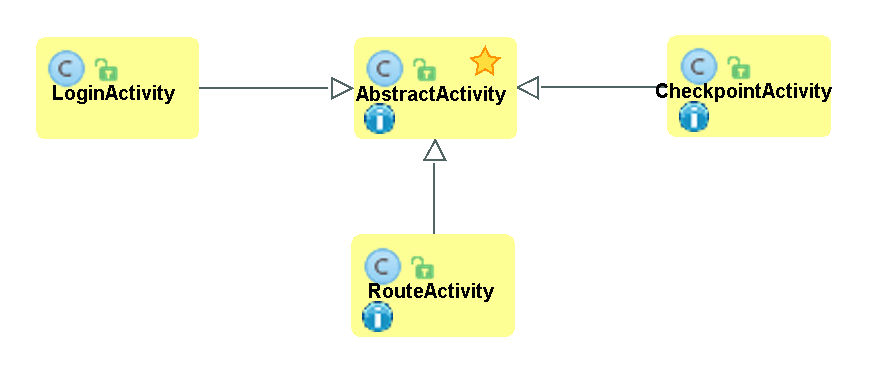
\includegraphics[scale=0.4]{\imagesRoot/abstract_activity_hierarchy.PNG}
	\caption
	{Klassenhierarchie der Klasse \emph{AbstractActivity}}
\end{figure}
\ \newline
Folgende Abbildung zeigt die Paketstruktur der Anwendung \emph{AmazingRace}. Als Wurzelnamensraum wurde \emph{at.fh.ooe.moc5.amazingrace} gewählt unter dem sich alle Ressourcen befinden.
\begin{figure}[h]
	\centering
	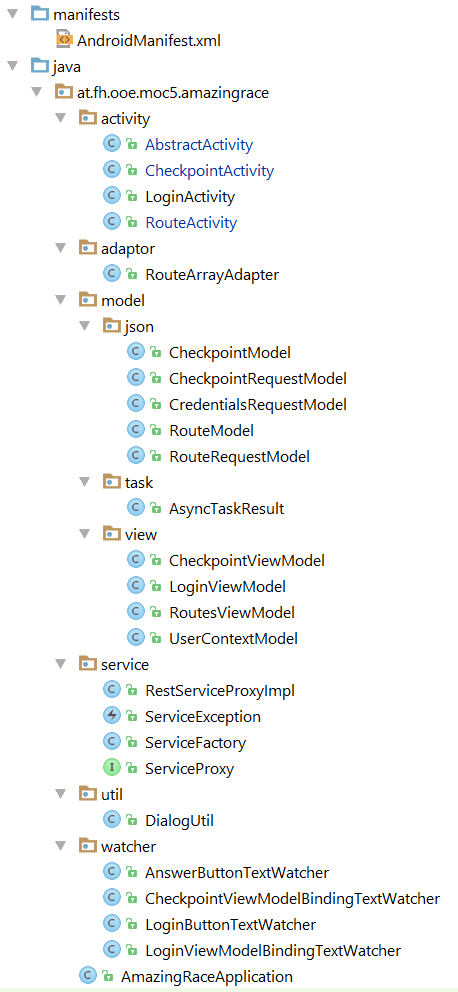
\includegraphics[scale=0.65]{\imagesRoot/amazingrace_package_structure.PNG}
	\caption
	{Paketstruktur der Anwendung}
\end{figure}
\ \newline
\newpage

Folgende Abbildung zeigt die Ressourcenverzeichnisse in denen alle Ressourcen wie \emph{Layout} usw. liegen. Es wurde hierbei darauf verzichtet, die Ressourcen für mehrere Endgeräte und Sprachen zu definieren.
\begin{figure}[h]
	\centering
	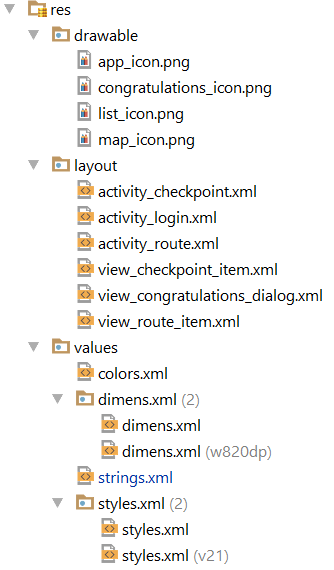
\includegraphics[scale=0.65]{\imagesRoot/amazingrace_resource_structure.PNG}
	\caption
	{Ressourcen der Anwendung}
\end{figure}
\ \newline
Des Weiteren wurde eine Klasse \emph{AmazingRaceApplication} eingeführt, die die unbehandelten Exceptions behandelt, den Benutzerkontext hält und gemeinsam verwendete Konstanten definiert.
\newline
\newpage

\subsection{Source}
Im folgenden ist der gesamte Source der Anwendung aufgeführt.

\subsubsection{Manifest}
\begin{code}
	\caption{AndroidManifest.xml}
	\xmlSourceFile{\manifestsRoot/AndroidManifest.xml}
\end{code}
\newpage
\subsubsection{Aktivitäten}
\begin{code}
	\caption{AmazingRaceApplication.java}
	\javaSourceFile{\javaRoot/AmazingRaceApplication.java}
\end{code}
\newpage
\begin{code}
	\caption{AbstractActivity.java}
	\javaSourceFile{\activityRoot/AbstractActivity.java}
\end{code}
\newpage
\begin{code}
	\caption{LoginActivity.java}
	\javaSourceFile{\activityRoot/LoginActivity.java}
\end{code}
\newpage
\begin{code}
	\caption{RouteActivity.java}
	\javaSourceFile{\activityRoot/RouteActivity.java}
\end{code}
\newpage
\begin{code}
	\caption{CheckpointActivity.java}
	\javaSourceFile{\activityRoot/CheckpointActivity.java}
\end{code}
\newpage

\subsubsection{Adapter}
\begin{code}
	\caption{RouteArrayAdapter.java}
	\javaSourceFile{\adapterRoot/RouteArrayAdapter.java}
\end{code}
\newpage

\subsubsection{JSON-Models}
\begin{code}
	\caption{CheckpointModel.java}
	\javaSourceFile{\jsonModelRoot/CheckpointModel.java}
\end{code}
\newpage
\begin{code}
	\caption{CheckpointRequestModel.java}
	\javaSourceFile{\jsonModelRoot/CheckpointRequestModel.java}
\end{code}
\newpage
\begin{code}
	\caption{CredentialsRequestModel.java}
	\javaSourceFile{\jsonModelRoot/CredentialsRequestModel.java}
\end{code}
\newpage
\begin{code}
	\caption{RouteModel.java}
	\javaSourceFile{\jsonModelRoot/RouteModel.java}
\end{code}
\newpage
\begin{code}
	\caption{RouteRequestModel.java}
	\javaSourceFile{\jsonModelRoot/RouteRequestModel.java}
\end{code}
\newpage

\subsubsection{Task-Models}
\begin{code}
	\caption{AsyncTaskResult.java}
	\javaSourceFile{\taskModelRoot/AsyncTaskResult.java}
\end{code}
\newpage

\subsubsection{View-Models}
\begin{code}
	\caption{LoginViewModel.java}
	\javaSourceFile{\viewModelRoot/LoginViewModel.java}
\end{code}
\newpage
\begin{code}
	\caption{RoutesViewModel.java}
	\javaSourceFile{\viewModelRoot/RoutesViewModel.java}
\end{code}
\newpage
\begin{code}
	\caption{UserContextModel.java}
	\javaSourceFile{\viewModelRoot/UserContextModel.java}
\end{code}
\newpage
\begin{code}
	\caption{CheckpointViewModel.java}
	\javaSourceFile{\viewModelRoot/CheckpointViewModel.java}
\end{code}
\newpage

\subsubsection{Service}
\begin{code}
	\caption{ServiceProxy.java}
	\javaSourceFile{\serviceRoot/ServiceProxy.java}
\end{code}
\newpage
\begin{code}
	\caption{RestServiceProxyImpl.java}
	\javaSourceFile{\serviceRoot/RestServiceProxyImpl.java}
\end{code}
\newpage
\begin{code}
	\caption{ServiceException.java}
	\javaSourceFile{\serviceRoot/ServiceException.java}
\end{code}
\newpage
\begin{code}
	\caption{ServiceProxyFactory.java}
	\javaSourceFile{\serviceRoot/ServiceProxyFactory.java}
\end{code}
\newpage

\subsubsection{Utilities}
\begin{code}
	\caption{DialogUtil.java}
	\javaSourceFile{\utilRoot/DialogUtil.java}
\end{code}
\newpage

\subsubsection{Watcher}
\begin{code}
	\caption{AnswerButtonTextWatcher.java}
	\javaSourceFile{\watcherRoot/AnswerButtonTextWatcher.java}
\end{code}
\newpage
\begin{code}
	\caption{CheckpointViewModelBindingTextWatcher.java}
	\javaSourceFile{\watcherRoot/CheckpointViewModelBindingTextWatcher.java}
\end{code}
\newpage
\begin{code}
	\caption{LoginButtonTextWatcher.java}
	\javaSourceFile{\watcherRoot/LoginButtonTextWatcher.java}
\end{code}
\newpage
\begin{code}
	\caption{LoginViewModelBindingTextWatcher.java}
	\javaSourceFile{\watcherRoot/LoginViewModelBindingTextWatcher.java}
\end{code}
\newpage

\subsection{Layout}
\begin{code}
	\caption{activity\_login.xml}
	\xmlSourceFile{\layoutRoot/activity_login.xml}
\end{code}
\newpage
\begin{code}
	\caption{activity\_route.xml}
	\xmlSourceFile{\layoutRoot/activity_route.xml}
\end{code}
\newpage
\begin{code}
	\caption{activity\_checkpoint.xml}
	\xmlSourceFile{\layoutRoot/activity_checkpoint.xml}
\end{code}
\begin{code}
	\caption{view\_checkpoint\_item.xml}
	\xmlSourceFile{\layoutRoot/view_checkpoint_item.xml}
\end{code}
\newpage
\begin{code}
	\caption{view\_route\_item.xml}
	\xmlSourceFile{\layoutRoot/view_route_item.xml}
\end{code}
\begin{code}
	\caption{view\_congratulations\_dialog.xml}
	\xmlSourceFile{\layoutRoot/view_congratulations_dialog.xml}
\end{code}
\newpage

\subsection{Values}
\begin{code}
	\caption{strings.xml}
	\xmlSourceFile{\valuesRoot/strings.xml}
\end{code}
\newpage
\end{document} 